\Exhibit{ComposerWikipedia}{%
    Wikipedia article on `Composer (Software)' that confirms the address of `Packagist' repository%
}

This is a screenshot of the Wikipedia page on `Composer (Software)'.
The point on this page is the explanation what `Packagist' is in software
(because Packagist does not have a dedicated Wikipedia page).

This page mentions:

\Quote{%
    Composer runs from the command line and installs dependencies (e.g. libraries) for an application.
    It also allows users to install PHP applications that are available on `Packagist'[5]
    which is its main repository containing available packages.%
}

This proves that Packagist is the main source of PHP packages
and thus is a proper source of usage statistics for them.

The link at the bottom of the page (numbered 5) points to packagist.org
which is the source of statistics in \ExhibitRef{PhpStanPackagist}.

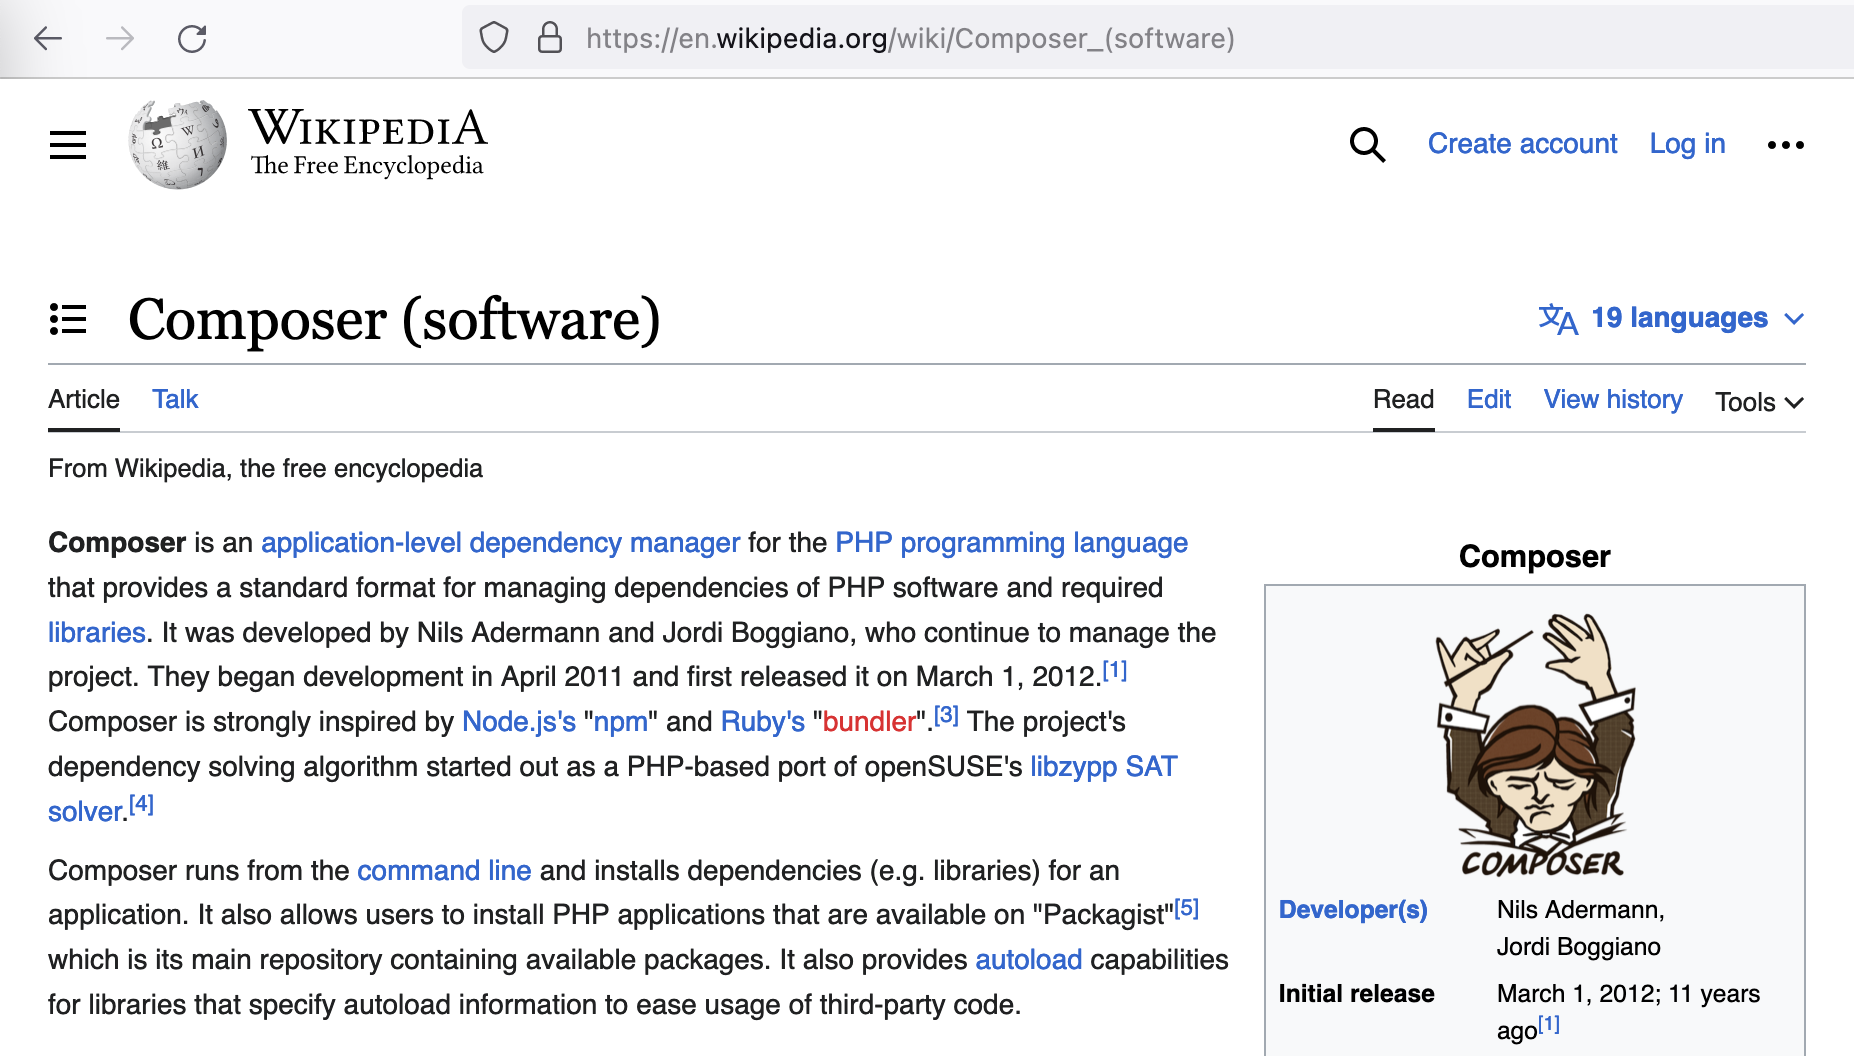
\includegraphics[width=\textwidth]{packagist-wikipedia-p1}
\CenterParentheses{Middle part skipped}

\pagebreak

\CenterParentheses{Middle part skipped}
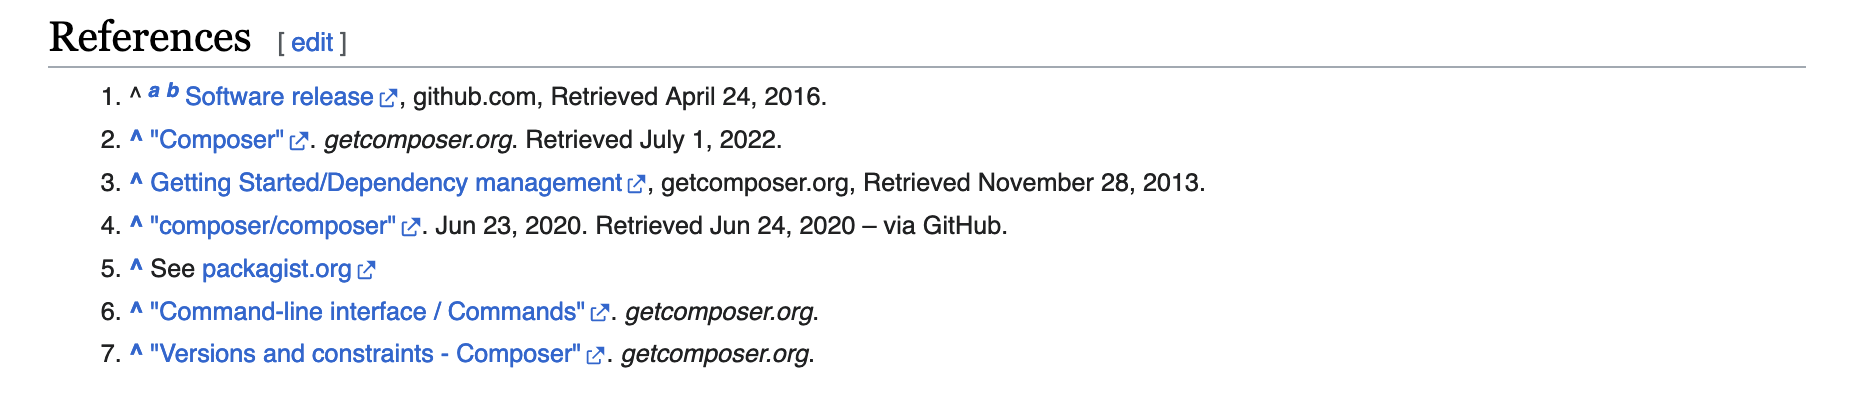
\includegraphics[width=\textwidth]{packagist-wikipedia-bottom}

\pagebreak




